A perturbációszámításhoz a Hamilton operátort két részre bontom fel:
\begin{equation}
	\op{H} = \op{H}_0 + \op{V}
\end{equation}
A $\op{H}_0$ operátorhoz tartozó rezolvens $\op{G}_0\left(E\right)$. $\op{H}$ és $\op{H}_0$ kifejezhetőek a rezolvenseikkel. Ha a kifejezéseket behelyettesítjük a fenti egyenletbe, implicit egyenletet kapunk $op{G}\left(E\right)$-re nézve, melyet fel lehet használni perturbációszámításra. Az egyenletet balról $\op{G}_0^{-1}\left(E\right)$-vel, jobbról $\op{G}^{-1}\left(E\right)$-vel szorzunk.
\begin{equation}
	\op{G}^{-1}\left(E\right) + E = \op{G}_0^{-1}\left(E\right) + E + \op{V}
\end{equation}
\begin{equation}
	\op{G}\left(E\right) = \op{G}_0\left(E\right) - \op{G}_0\left(E\right)\op{V}\op{G}\left(E\right)
	\label{green:pertmaster}
\end{equation}
Az alábbi módon definiálva $\op{G}_n\left(E\right)$ operátort, \aref{green:pertmaster}. egyenlethez hasonló rekurziós összefüggés áll fent:
\begin{equation}
	\op{G}_n\left(E\right) = \op{G}_0\left(E\right)\sum_{k=0}^n\left(-\op{V}\op{G}_0\left(E\right)\right)^k
\end{equation}
\begin{equation}
	\op{G}_{n+1}\left(E\right) = \op{G}_0\left(E\right) - \op{G}_0\left(E\right)\op{V}\op{G}_n\left(E\right)
\end{equation}
Ha $\norm{\op{V}\op{G}_0\left(E\right)} < 1$ akkor a $\op{G}_n$ sorozat konvergál, és kielégíti \aref{green:pertmaster}. egyenletet. Ezért konvergencia esetén:
\begin{equation}
	\op{G}\left(E\right) = \op{G}_0\left(E\right)\sum_{n=0}^\infty\left(-\op{V}\op{G}_0\left(E\right)\right)^n
\end{equation}
A perturbbálatlan operátornak a lineáris potenciál nélküli dobozba zárt részecske Hamilton operátorát választom, $\op{H}_0=\frac{1}{2m}\op{p}^2$, így a lineáris potenciál marad a perturbáció $\op{V} = F\op{x}$. A perturbálatlan $\op{G}_0\left(E\right)$ Green-függvényt is \aref{green:Cbegin}-\ref{green:Cend}, \ref{green:xy}. és \aref{green:yx}. egyenletek alapján határozom meg.
\begin{equation}
	G_0\left(x,y;E\right) =
	\begin{cases}
		-\frac{2m}{k\hbar^2}\frac{1}{\sin\left(kL\right)} \sin\left(k\left(y-L\right)\right)\sin\left(kx\right) & x\leq y\\
		-\frac{2m}{k\hbar^2}\frac{1}{\sin\left(kL\right)} \sin\left(k\left(x-L\right)\right)\sin\left(ky\right) & x>y\\
	\end{cases}
\end{equation}
, ahol $k = \frac{\sqrt{2mE}}{\hbar}$.
\begin{figure}[H]
	\centering
	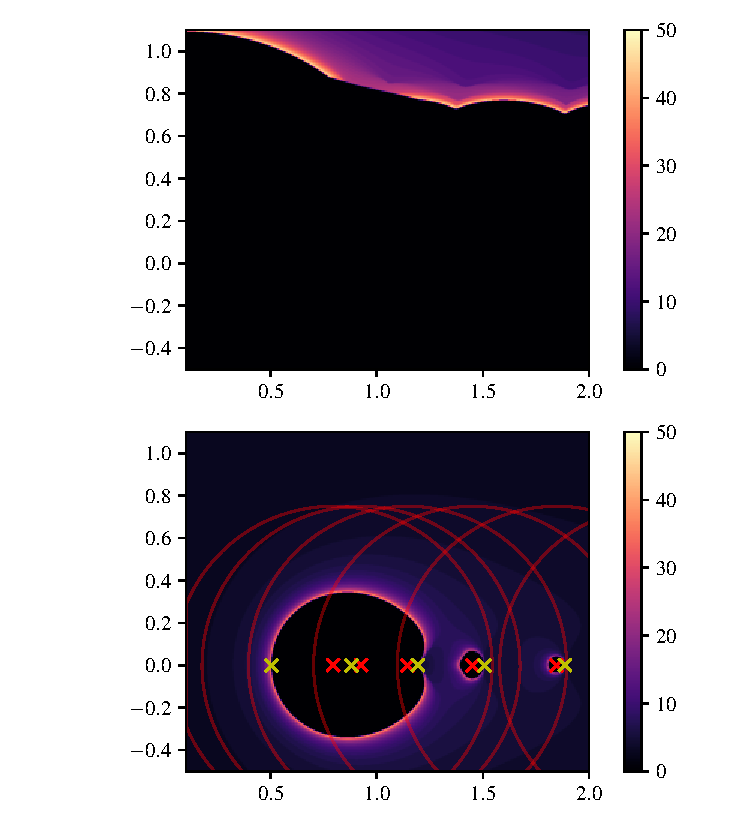
\includegraphics[scale=1]{./figs/convergence3.pdf}
	\caption[Green-függvény perturbációs sorának konvergenciája]{Ez az ábra a két perturbációs sor konvergenciáját hasonlítja össze a komplex energia síkon. A felső ábra a $V=Fx$ perturbáló potenciálnak, míg az alsó a $V = Fx-FL/2$ perturbáció szerinti sornak felel meg. A fekete tartományok divergenciát jelölnek, míg a többi szín a sorfejtés tagjainak csökkenési sebességét jellemzik, a norma harmadolásához szükséges lépések számát megadva. A piros körökön kívüli tartomány a ?? formula által garantált konvergencia tartományát jelöli. A piros x-ek a $\hat{G}_0$ pólusait, a sárga x-ek pedig az egzakt $\hat{G}$ operátor pólusait jelölik.}
\end{figure}